%%%%%%%%%%%%%%%%%%%%%%%%%%%%%%%%%%%%%%%%%
% Short Sectioned Assignment
% LaTeX Template
% Version 1.0 (5/5/12)
%
% This template has been downloaded from:
% http://www.LaTeXTemplates.com
%
% Original author:
% Frits Wenneker (http://www.howtotex.com)
%
% License:
% CC BY-NC-SA 3.0 (http://creativecommons.org/licenses/by-nc-sa/3.0/)
%
%%%%%%%%%%%%%%%%%%%%%%%%%%%%%%%%%%%%%%%%%

%------------------------------------------------------------------------------
%	PACKAGES AND OTHER DOCUMENT CONFIGURATIONS
%------------------------------------------------------------------------------

\documentclass[paper=a4, fontsize=11pt]{scrartcl} % A4 paper and 11pt font size

\usepackage[T1]{fontenc} % Use 8-bit encoding that has 256 glyphs
%\usepackage{fourier} % Use the Adobe Utopia font for the document - comment this line to return to the LaTeX default
\usepackage[swedish]{babel} % English language/hyphenation
\usepackage{amsmath,amsfonts,amsthm} % Math packages

\usepackage[font=scriptsize,labelfont=bf]{caption}
\usepackage{verbatim}
\usepackage{hyperref}
\usepackage[utf8]{inputenc} % Needed to support swedish "åäö" chars
\usepackage{titling} % Used to re-style maketitle
\usepackage{enumerate}
\usepackage{lipsum} % Used for inserting dummy 'Lorem ipsum' text into the template

\usepackage{tabularx}
\usepackage{hyperref}
\usepackage{url}
\usepackage{graphicx}
\usepackage[left=2.5cm, right=2.5cm]{geometry} % margins for title page. changed below.

\usepackage{sectsty} % Allows customizing section commands
\allsectionsfont{\normalfont} % Make all sections centered, the default font and small caps

\usepackage{fancyhdr} % Custom headers and footers
\pagestyle{fancyplain} % Makes all pages in the document conform to the custom headers and footers
\fancyhead{} % No page header - if you want one, create it in the same way as the footers below
\fancyfoot[L]{} % Empty left footer
\fancyfoot[C]{} % Empty center footer
\fancyfoot[R]{\thepage} % Page numbering for right footer
\renewcommand{\headrulewidth}{0pt} % Remove header underlines
\renewcommand{\footrulewidth}{0pt} % Remove footer underlines
\setlength{\headheight}{13.6pt} % Customize the height of the header

\numberwithin{equation}{section} % Number equations within sections (i.e. 1.1, 1.2, 2.1, 2.2 instead of 1, 2, 3, 4)
\numberwithin{figure}{section} % Number figures within sections (i.e. 1.1, 1.2, 2.1, 2.2 instead of 1, 2, 3, 4)
\numberwithin{table}{section} % Number tables within sections (i.e. 1.1, 1.2, 2.1, 2.2 instead of 1, 2, 3, 4)

\setlength\parindent{0pt} % Removes all indentation from paragraphs - comment this line for an assignment with lots of text

\usepackage{fancyvrb}
\DefineShortVerb{\|}


\posttitle{\par\end{center}} % Remove space between author and title
%----------------------------------------------------------------------------------------
% TITLE SECTION
%----------------------------------------------------------------------------------------

\title{ 
\huge Laboration 3 \\ Minneshantering v. 4 \\ % The assignment title
\vspace{10pt}
\normalfont \normalsize 
\textsc{ID2200 - Operating Systems } \\ [25pt] %
}

\author{Gustaf Lindstedt \\ glindste@kth.se \\ 910301-2135 \and Martin Runelöv \\ mrunelov@kth.se \\ 900330-5738}

\date{\vspace{8pt}\normalsize\today} % Today's date or a custom date

\begin{document}

\maketitle

%------------------------------------------------------------------------------
\section{Inledning}

% OBS! Se till så att filerna är läsbara för assistenterna (se 3.4 ).
Koden, inklusive testkod, finns tillgänglig i följande sökväg:\\
|/afs/ict.kth.se/home/m/r/mrunelov/os/lab3/|. \\

I appendix finns källkoden för |malloc.c|, |malloc.h| samt testfilerna |malloc_test_small.c|,\\ |malloc_test_big.c|, och |malloc_test_rand.c|. \\

Körinstruktioner finns i filen README.md\\

Följande ändringar har gjorts i testfilerna:\\
-- Shebangen i |RUN_TESTS| har ändrats från |#!/bin/csh| till |#!/bin/bash|.\\
-- |#include <sys/types.h>| las till i |tstcrash_complex.c| för att kunna
använda typen |caddr_t|.


% Verksamhetsberättelse och synpunkter på laborationen. Beskriv arbetets utveckling. Hade du problem med verktygen,
% kompilatorn m.fl.? Hur lång tid har arbetet tagit? Skriv dina förslag till förändringar, idéer etc. Tyck fritt! 
% Vi är angelägna om att få respons, så att vi kan förbättra till nästa år.

% Uppskattning av tidsåtgång och eventuella kommentarer kring laborationen
\subsection{Verksamhetsberättelse}

Vi började genom att studera implementationen i The C Programming language.
Den användes som mall och rättesnöre när vi implementerade vår egna.
Efter att malloc och free implementerats implementerade vi realloc som
utnyttjade dom.
När dessa delar klarade sina tester implementerade vi både Best-fit och
Worst-fit algoritmerna för malloc.
Den sista stora additionen till vår implementation var att vi började hålla
reda på även allokerade areor och inte bara lediga utrymmen.
Detta för att kunna identifiera felaktiga anrop till free. \\

Resten av tiden har spenderats på att förfina tester och skript för att kunna
sammanställa grafer och att utvärdera algoritmerna.\\

Vi uppskattar att den totala tidsåtgången för den här laborationen har varit
ca 20h.\\


\subsection{Synpunkter}
gprof fungerar inte längre på Mac OS X, och skolans datorer ger en inte
tillräckligt med minne för att göra utförliga tester med gprof.
Dessutom skulle vi uppskatta om det fanns ett tydligt exempel på
gprof-användning då detta har en tendens att vara krångligt.\\

Det är lite förvirrande att systemets malloc har någon optimering som gör att
minnesåtgången blir 0 i alla tester. 
Detta kanske inte gäller alla system, men det borde kanske nämnas i labbpeket
för att göra folk beredda på det.\\

Testfilerna är väldigt otydliga med huruvida man har klarat ett test eller
inte. Om man kollar i källkoden kan man oftast räkna ut vad som menas, men det
borde inte behövas.
Precis som MERGE-testet borde samtliga tester avslutas med antingen
|Test passed OK| eller |Test failed|.
En sådan text per deltest vore ännu bättre.\\

Det är även förvirrande med texten |worst case calculation| i MEMORY-testet.
Det verkar som att $> 2.0*\text{worst-case}$ anses vara ett misslyckande, men
man får lätt intrycket att man ska ligga $< 1.0$.


\section{Förberedelsefrågor}

\subsection*{mmap:}

Adress-parametern till |mmap| specificerar en virtuell adress som är ett
förslag till var |mmap| ska skapa en ny mappning.
|mmap| kommer att skapa en mappning på en närliggande sida.
Om adressen är |NULL| väljer mmap själv var minnet allokeras.\\

Om |__endHeap| inte skulle initialiseras till |sbrk(0)| skulle minnet fortfarande
allokeras, men alla allokeringar efter den första skulle ge sämre förslag till
|mmap| eftersom de utgår från minnesadress 0 istället för starten på heapen.
Detta problem kan även uppstå med |sbrk(0)| eftersom |mmap| inte garanterar att
mappningen sker till den specificerade adressen.\\

|mmap| returnerar en pekare till det mappade området, eller |MAP_FAILED| om
mappningen misslyckades.\\

Man måste specificera någon av flaggorna |MAP_SHARED| eller |MAP_PRIVATE|.
|MAP_SHARED| innebär att uppdateringar av mappningen är synlig för andra
processer som har samma mappning.
|MAP_PRIVATE| skapar en privat copy-on-write-mappning som inte skriver igenom
till det mappade området.

%------------------------------------------------------------------------------
\section{Problembeskrivning}
Uppgiften gick ut på att skriva egna implementationer av systemfunktionerna
|malloc|, |free| och |realloc|.
Funktionen |malloc| allokerar nytt minne för använding av programmet, medan
|free| friar allokerat minne så att det kan återanvändas.
Funktionen |realloc| tar allokerat minne och utökar eller minskar det till
önskad storlek.
Finns det inte plats för att utöka utrymmet så allokerar |realloc| nytt minne
och friar det gamla blocket, med kravet att informationen i det gamla blocket
flyttas till det nya blocket så att data inte förstörs.
Bland kraven ingick att det inte fick förekomma några minnesläckor.



%------------------------------------------------------------------------------
\section{Programbeskrivning}

% Har nästan förstått det här. Men är lite osäker på vad dom vill.
% Det nedan + motsvarande förberedelsefrågor-del kan ses som anteckningar tills vidare...
%
% Det är lite oklart hur det hela ska funka.
% sbrk ger oss program break, men __endHeap med mmap håller bara reda på 
% mängden mappat minne. Den bryr sig inte om luckor osv. Se request_memory.
%
Om |MMAP| är definierad deklareras en variabel |__endHeap| samt funktionen 
|void *endHeap(void)| som initialiserar |__endHeap| om den är |NULL| och
returnerar |__endHeap|.\\

|__endHeap| används som adress-parameter till |mmap| när |malloc| begär 
mer minne av operativsystemet via |request_memory|.

\subsection{Minnesblock}
I början av varje block ligger alltid en header som innehåller storleken på
blocket (inklusive headern) i antal headers samt en pekare till nästföljande
header.
Block är även alltid alignade till |sizeof(header)| som är storleken av en
|double| vilket brukar vara den största typen i C.

\subsection{Att hålla reda på minnesblock}

För att hålla reda på lediga block som har mappats men ej allokerats använder
sig implementationen av en länkad lista med headers till fria block.
Denna lista refereras till med hjälp av pekaren |free_list| som pekar på en
header till ett fritt block.
Varje gång ett block frias så länkas den in i listan på rätt plats med avseende
på minnesadress.
För att undvika att en användare kraschar programmet om hen försöker fria en
minnesadress som inte är början på ett allokerat block använder
implementationen även en länkad lista mellan allokerade block.
När |free| anropas så kontrolleras att den givna adressen ligger precis efter
en header till ett allokerat block genom att loopa igenom listan.
Listan refereras till genom pekaren |malloced_headers| som pekar på en header
till ett allokerat block.

\subsection{Malloc}
|malloc| tar en önskad storlek i bytes och returnerar adressen till början på
det nyallokerade minnet.
Ger man 0 som argument, eller ger ett värde större än maxvärdet för |long|
returnerar den |NULL|.
|malloc| letar först efter minne genom att loopa över |free_list| för att se om
det redan finns en tillräckligt stor mappad minnesarea för allokeringen.
Om en sådan hittas så länkas headern på blocket ur från |free_list| och länkas
in i |malloced_headers|.
Om ett tillräckligt stort block inte hittas så anropas funktionen
|request_memory| som använder |mmap| för att mappa ny minnesarea som sedan
länkas in i |free_list|.
\subsubsection{Algoritmer}
Som standard används First-fit, som allokerar första blocket som den hittar
som är tillräckligt stort.
Med hjälp av kompileringsflaggor kan |malloc| istället använda sig av Best-fit
eller Worst-fit.
Båda dessa algoritmer går igenom hela listan av fria block, men sparar en
pekare till det bästa respektive värsta blocket med avseende på hur bra det
passar den begärda storleken.
När alla fria block har undersökts används det bästa/värsta blocket som hittats
för allokeringen.

\subsection{Free}
|free| tar en adress till början av ett allokerat block och frigör minnet så
att det kan allokeras igen.
Om man ger en adress som är |NULL| eller som inte är början på ett allokerat
block görs ingenting.
|free| hämtar först headern till det allokerade blocket.
Därefter loopar den över listan av fria block för att leta reda på rätt plats
att länka in blocket på med avseende på minnesadress.
För att effektivisera minnesanvändningen så görs hopslagning av lediga block
som ligger bredvid varandra i minnet.
När |free| har hittat var det nya friade blocket ska länkas in så görs en koll
om blocket framför i listan gränsar till det nya blocket och om blocket
efter i listan gränsar till det nya blocket.

\subsection{Realloc}
|realloc| tar adressen till början av ett redan allokerat minnesområde samt
en önskad storlek i bytes som området antingen ska krympas till eller utökas
till.
Returvärdet är startadressen till det allokerade blocket (som kan ha flyttats).
Om man ger |NULL| som adress så görs bara ett anrop till |malloc|.
Om man ger 0 som storlek så görs bara ett anrop till |free|.
Om den önskade storleken är mindre än den nuvarande storleken minskas blockets
storlek och en ny header skapas vid den nya slutpunkten, varefter |free| anropas på
det nya blocket.
Då den begärda storleken är större än den nuvarande så görs ett anrop till
|malloc|, varefter minnet i det gamla blocket kopieras till det nya blocket
med hjälp av |memcpy|.
Därefter frias det gamla blocket med ett anrop till |free|.


%------------------------------------------------------------------------------
\section{Utvärdering}

Testerna gjordes med en page size på 4096 byte.\\

Tiden för en körning mättes med kommandot |time|, där |user time| användes,
vilket mäter tiden då en process befann sig i |user mode|.\\

Testerna utfördes genom att upprepade gånger allokera små mängder minnen.
Ett enskilt test gjordes med en minnesstorlek.
Denna minnesstorlek allokerades sedan enligt mönstret nedan:

\begin{verbatim}
for(i = 0; i < LOOPS; ++i) {
    for(j = 0; j < SIZE; ++j) {
        arr[j] = malloc(memory_size);
    }
}
\end{verbatim}

Utöver detta anropas |free| på allt allokerat minne i slutet på varje test.

I graferna nedan visas tiden i millisekunder på y-axeln och storleken på 
de allokerade blocken på x-axeln. När det allokerade minnet är en multipel
av pagesize visas denna multipel istället för antal byte.

\captionsetup{labelsep=newline}

\subsection{Stora allokeringar}

\begin{minipage}{.3\textwidth}
    \centering
    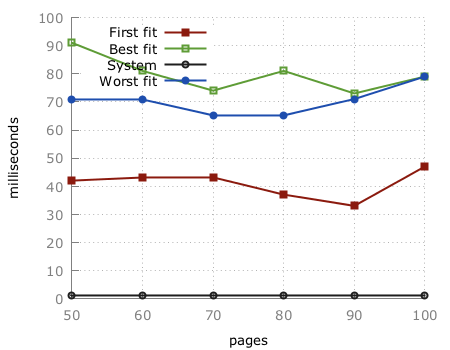
\includegraphics[width=1\textwidth]{images/time_plot_big1.png}
    \label{fig:big1}
    \captionof{figure}{\tiny{LOOPS = 10, SIZE = 128}}
\end{minipage}%
\begin{minipage}{.3\textwidth}
    \centering
    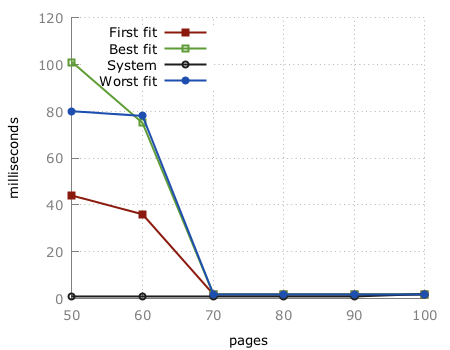
\includegraphics[width=1\textwidth]{images/time_plot_big2.png}
    \label{fig:big2}
    \captionof{figure}{\tiny{LOOPS = 10, SIZE = 128}}
\end{minipage}
\begin{minipage}{.3\textwidth}
    \centering
    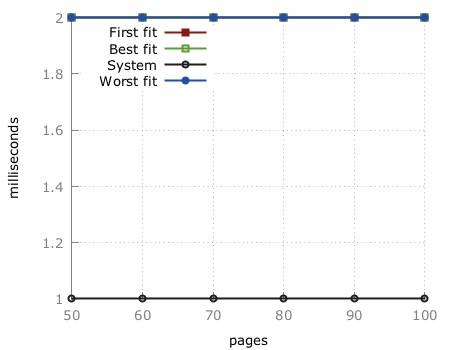
\includegraphics[width=1\textwidth]{images/time_plot_big3.png}
    \label{fig:big3}
    \captionof{figure}{\tiny{LOOPS = 10, SIZE = 128}}
\end{minipage}\\\\

För att testa algoritmernas effektivitet vid större allokeringar har vi utfört
tester där multipler av page size (4096) allokeras. I figur 5.1 kan man se en
tidsjämförelse mellan de olika algoritmerna. Anledningen till att first fit är 
något snabbare än best och worst fit kan förklaras av den overhead som finns i 
best och worst fit när de loopar igenom |free_list|.
% KOMMENTERA MER?...lite vag.

Systemets malloc presterar väldigt bra och ligger stabilt på 1 millisekund.
Våra algoritmer får däremot ett värstafallsscenario. Vi allokerar ett jämnt
antal pages varje gång, vilket med headern inräknat leder till att vi begär
lite mer minne än vad som efterfrågas. Detta innebär alltså att små hål
skapas i minnet och |free_list| fylls med dessa, vilket sänker prestandan
i samtliga algoritmer.\\

I figur 5.2 visas en version av samma test där |mmap|-anropet har modifierats
så att det begär mer minne än vad som efterfrågades. Detta betyder att man 
antar att det kommer att begäras mer minne inom kort. Resultatet av detta kan
ses i figur 5.2 där denna mekanism börjar användas för page size $>= 70$ .
Effekten blir en rejäl förändring i hastighet där våra algoritmer närmar sig
system malloc. De stabiliserar sig på 2 millisekunder. Detta har sin förklaring
i att den overhead som |mmap|-anrop innebär nästan helt försvinner.
Våra algoritmer är dock fortfarande dubbelt så långsamma som systemets malloc.\\

I figur 5.3 har vi subtraherat |sizeof(header)| från varje malloc-anrop.
Det innebär att vi kommer att använda allt minne vi får av |mmap| och undviker
därmed fragmentering. Detta ger samma resultat som i 5.2.
Detta kan ses som ett bästafall för algoritmerna, där fragmentering motverkats
genom att specialanpassa storleken på minnet som allokeras. Detta är dock inte
särskilt realistiskt då storlekarna har skräddarsytts till att vara perfekta.
I ett verkligt system är det väldigt svårt att hålla nere fragmenteringen
av minnet.


\subsection{Små allokeringar}

\begin{minipage}{.5\textwidth}
    \centering
    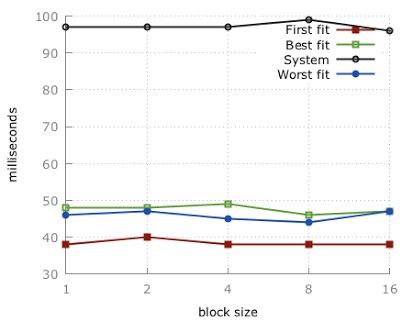
\includegraphics[width=1\textwidth]{images/time_plot_small1.png}
    \label{fig:small1}
    \captionof{figure}{\tiny{LOOPS = 20000, SIZE = 128}}
\end{minipage}%
\begin{minipage}{.5\textwidth}
    \centering
    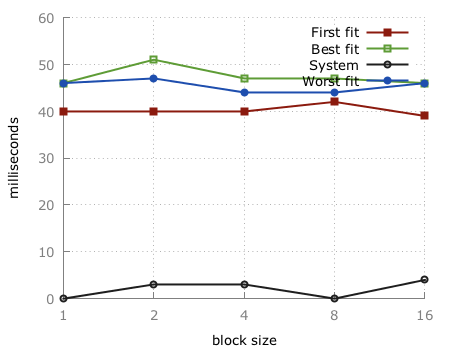
\includegraphics[width=1\textwidth]{images/time_plot_small2.png}
    \label{fig:small2}
    \captionof{figure}{\tiny{LOOPS = 20000, SIZE = 128}}
\end{minipage}\\\\

I detta test allokerade vi väldigt små mängder minne väldigt många gånger.
Vi loopade 20 000 gånger och allokerade minne till en
array av längd 128 i varje iteration.\\
Resultaten av två identiska körningar kan ses i figur 5.4 och 5.5.\\

First fit var något snabbare än best och worst fit. Detta beror antagligen på
att vi under en och samma körning allokerar minnen av samma storlek. Detta 
innebär att first fit ofta får samma mängd fragmentering som best och worst fit,
men med färre iterationer i |free_list|.\\

Som man kan se i figurerna hade systemets malloc ojämn prestanda vid små allokeringar.
Den dåliga körningstiden skulle bland annat kunna förklaras av att allokeringar
av så små minnen är väldigt ovanligt.
Systemets malloc innehåller dessutom en hel del funktionalitet som kräver
initiering och hushållning.\\


\subsection{Slumpmässiga allokeringar}
För att vidare simulera vanlig användning körde vi ett test där vi allokerade
slumpmässiga minnesstorlekar.
Man ser då en tydlig skillnad mellan de olika algoritmerna, där first-fit
klarar sig bäst vid simulerad s.k. ``vanlig'' användning.\\

\begin{minipage}{.5\textwidth}
    \centering
    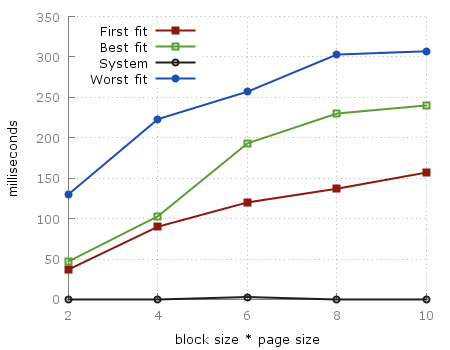
\includegraphics[width=1\textwidth]{images/time_plot_rand.png}
    \label{fig:p3}
    \captionof{figure}{\tiny{LOOPS = 20, SIZE = 128}}
\end{minipage}\\

Grafen visar hur algoritmerna presterar då man ökar storleken för hur stora
allokeringarna får vara.
Storleken på en minnesallokering beräknades genom formeln
|multiple*(rand()%pagesize)|, och varierade alltså från 0 till
|multiple*pagesize|.


\subsection{Skydd av minne}

Vi implementerade skydd mot sönderskrivning av våra kontrollstrukturer. 
Detta åstadkom vi genom att ha en separat lista som håller reda på minne som
|malloc| har allokerat.
Varje gång |free| anropas kontrolleras dess header genom att loopa över denna
lista.
Om blocket inte finns i listan returneras |NULL|.


\renewcommand{\refname}{\normalfont\selectfont\normalsize Referenser} 
\newpage
\begin{thebibliography}{9}

\bibitem{khernigan_ritchie}
Kernighan, Richie, 
\emph{''The C Programming Language''},
 andra upplagan,\\ Prentice Hall, 
 1988,
 s. 185- 189.

\bibitem{malloc}
malloc(3) - Linux man page -
\url{http://linux.die.net/man/3/malloc}

\bibitem{mmap}
mmap(2) - Linux man page -
\url{http://linux.die.net/man/2/mmap}

\bibitem{sbrk}
sbrk(2) - Linux man page -
\url{http://linux.die.net/man/2/sbrk}


\end{thebibliography}


%------------------------------------------------------------------------------
\newpage
\section*{Appendix}
\subsection*{malloc.c}
\verbatiminput{../malloc.c}

\newpage
\subsection*{malloc.h}
\verbatiminput{../malloc.h}

\newpage
\subsection*{malloc\_test\_small.c}
\verbatiminput{../malloc_test_small.c}

\newpage
\subsection*{malloc\_test\_big.c}
\verbatiminput{../malloc_test_big.c}

\newpage
\subsection*{malloc\_test\_rand.c}
\verbatiminput{../malloc_test_big.c}


\end{document}
